\section{Importing data - Zhi Jiang}
My portion is to import data from data storage into a database in this project. Specifically, we need to read the file containing data in S3 and then import these data into a specified table in DynamoDB. In this portion, there are three main parts. First of all, I am going to describe what problems that have impeded my progress and my solutions for them. Secondly, I am going to talk about how I implement functions of my portion individually. Thirdly,  I am going to discuss what I plan to improve on my portion.

\subsection{Problem and Solution}
When I start to do my portion, the primary I consider is what service I can use to operate these data between S3 and DynamoDB. The primary solution we decided in Technology Review document is we is EMR. The reason is EMR, as a managed cluster platform that simplifies running big data frameworks can provide many tools to process big data such as Hive and Pig efficiently. In my original plan, I would like to run Hive command on EMR cluster for my portion, but there are some problems I encountered. The first issue is I was not able to create an EMR cluster. Two necessary conditions are creating key pair and roles for creating a cluster, but the technical assistance of our client as an administrator did not authorize these two services for me at the initial stage. According to our communication, I got the permission of creating a key pair, but I still need to permission of setting up the role. Our administrator thought it would be equivalent to being system administrator if she gave me full access to create a role. She also told me she would try to use other ways to help resolve this problem, but in fact, I have wasted a lot of time on this part. Therefore, I started to consider other solution.\\ 

\noindent I went back to watch technology review document, and I planned to use an alternative solution, which is an AWS SDK for Python. According to my research, I believed Boto 3 as an AWS SDK for Python should be the most appropriate method to solve this problem. There are three benefits; one is I am familiar with Python, so I do not need to spend more time to learn it. Another is SDK provides useful methods which can quickly complete correlative tasks such as accessing S3 and DynamoDB. The third benefit the cost of this solution is less than the previous one because it does not require additional environment configuration like creating a cluster.

\subsection{Function Implementation}
When we implement this function,  I need to read data from a file stored in S3 and then import these data to a table in DyanmoDB firstly. I also spent lots of time on this part because I always used improper method until I found the correct one.  The following code is an inappropriate method I used before.

\begin{lstlisting}[language=Python, caption=inappropriate method to access S3 and read data]
	s3 = boto3. resource('s3')
	obj = s3.Object('bucket_name', 'file_name')
	content = obj.get()['Body'].read()  
\end{lstlisting}

\noindent I found this method in Boto 3 document. I was not familiar with this SDK, so I through each file should be regarded as an object, and then I just need to read the content of this object. But eventually, I failed to read data from variable “content.”  In fact, I did not completely understand the role of an object type in this SDK. Object type is a complex constructor, and it contains much information. I tried to find other solution. The difference between this two method is the file we want to process is loaded into a temporary file and extension of its text.

\begin{lstlisting}[language=Python, caption=appropriate method to access S3 and read data]
	s3 = boto3.resource('s3')
	s3.download_file("bucket_name", "file_name", "tmp.txt") 
\end{lstlisting}

\noindent The benefit of this approach is it made this problem more familiar to me because I have done many similar tasks, which I/O for a text file. So now what I should do was using a conventional method to read this temporary file in Python. When I wrote data in a table, there are two things I need to mention. One is I used method table.batch writer() to fo do it. The purpose of this approach is you can both speed up the process and reduce the number of write requests made to the service if you are loading a lot of data at a time, so it is very appropriate to this project related big data. Second is the primary key. The basic idea to create a table is that it must contain a primary key. The purpose of this way is to make each row unique. In our implementation, we set an int variable as primary key, and then to increase it as creating a new item.

\begin{lstlisting}[language=Python, caption=importing data]
	# open this file contains content of CSV
	f = open('tmp.txt')

	# set a variable as primary key
	num = 0

	# use table.batch_writer() method to load a lot of data
	with table.batch_writer() as batch:
		for line in f:
			num += 1
			list_line = line.split(',')
		
			# create a new item and put it into a table
			batch.put_item(
				Item = {
					'primarykey': str(num),
					'attribute_name0': list_line[0],
					'attribute_name1': list_line[1],
					...
					...
					...
				}
			)
	f.close()
\end{lstlisting}

\noindent We went to check results after we run this script. Fortunately, the result met our expectations. The following picture is showing the result of importing data. In this table "DataForCapstone", we can find the item count is 671, which means there are 671 items in our table. When we went to back check our CSV file, it still has 671 rows. So we successfully import data from S3 into DynamoDB.

 \begin{figure}[H]
 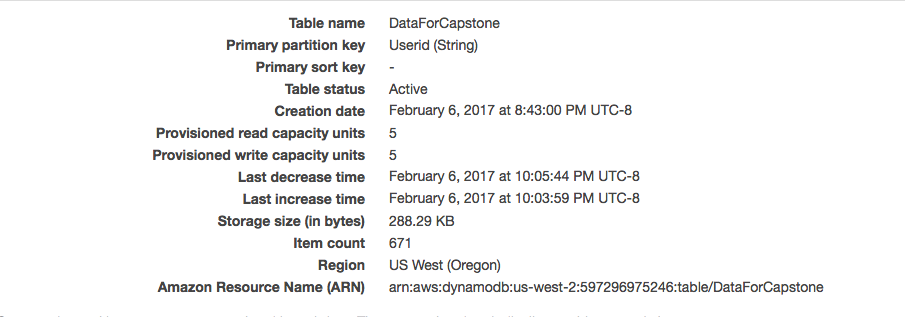
\includegraphics[width=17cm, height=8cm]{result.png}
 \centering
 \caption{\label{fig:4}result after importing data}
 \end{figure}

\subsection{Subsequent Improvement}
Although we have implement function of this part, we should improve our python script. Our current condition is that we need to create a table in Dynamo before importing data, in the other word, we import data into an existing table, but we hope our python script can create a table automatically as import data.\\

\noindent The one problem we have to encounter is the name of each attribute. In fact, the sample data file our client provided to us does not have a header, so we have to set a name of the attribute to each column according to our understanding. If a CSV file has a header includes all attribute name, we can use this header to create a table directly. Specifically, we can separate CSV files into two parts, one only includes a header, and another includes data. Then we just need to process part including a header for creating a table. 


